

%------------------------------------------
\subsection{First-order advection ODE in 1D}

What follows is borrowed from the book "Discontinuous finite elements in fluid dynamics and heat
transfer" by Ben Q. Li \cite{li06}.

To illustrate the basic ideas of the discontinuous finite element method, we
consider a simple, one-dimensional, first order differential equation with $u$
specified at one of the boundaries:
\begin{equation}
\frac{du}{dx} + g =0 \qquad x\in[a,b] \qquad \text{and} \qquad u(x=a)=u_a
\end{equation}
where $g$ is a constant (for simplicity).
The domain is discretized such that : $\Omega_j = [x_j,x_{j+1}]$ with $j = 1, 2, ..., nel$.
Then, integrating the above equation over the element $j$ with respect to a weighting function $f(x)$
\begin{equation}
\int_{x_j}^{x_{j+1}} \left( \frac{d u}{dx} + g \right) f(x) dx = 0
\end{equation}
Remembering that $\int_c^d u(x)v'(x) dx = [u(x)v(x)]_c^d - \int_c^d u'(x)v(x) dx$, 
we can now perform an integration by parts on the differential operator and we obtain:
\begin{equation}
[u(x)f(x)]_{x_j}^{x_{j+1}}  -\int_{x_j}^{x_{j+1}} \left( u \frac{d f}{dx} - g f(x)\right)  dx = 0
\end{equation}
or, 
\begin{equation}
u(x_{j+1})f(x_{j+1}) 
- u(x_{j})f(x_{j}) 
-\int_{x_j}^{x_{j+1}} \left( u \frac{d f}{dx} - g f(x)\right)  dx = 0
\end{equation}


On $\Omega_j$ $u$ is approximated by $u_h \in H$, $H$ being an appropriate function
space of finite dimension, and $f$ by $f_h$ taken from the same function space as $u_h$. 
Upon substituting $(u_h , f_h )$ for $(u,f)$ in the equation above, we have
the discontinuous Galerkin finite element formulation:
\begin{equation}
u_h(x_{j+1}) f_h(x_{j+1}) - u_h(x_{j})f_h(x_{j}) 
-\int_{x_j}^{x_{j+1}} \left( u_h \frac{d f_h}{dx} - g f_h(x)\right)  dx = 0
\end{equation}

In the continuous finite element approach, the field variable $u_h$ is forced to be
continuous across the boundary.
The essential idea for the discontinuous method is
that $u_h$ is allowed to be discontinuous across the boundary. Therefore, across the
element, the following two different values are defined at the two sides of the
boundary:
\begin{equation}
u_j^+ = \lim_{x \searrow x_j^+} u_h(x)
\qquad
u_j^- = \lim_{x \nearrow x_j^-} u_h(x)
\end{equation}

\begin{center}
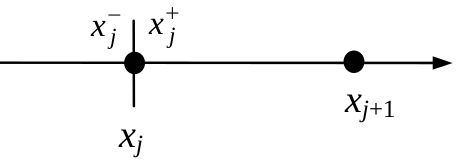
\includegraphics[width=4cm]{images/dgfem/dgfem_1}\\
{\scriptsize An illustration of the jump across $x_j$ of element $j$: 
$x_j$ and $x_{j+1}$ mark the
boundaries of the element}
\end{center}

Conversely, we also have:
\begin{equation}
u_{j+1}^+ = \lim_{x \searrow x_{j+1}^+} u_h(x)
\qquad
u_{j+1}^- = \lim_{x \nearrow x_{j+1}^-} u_h(x)
\end{equation}



It is key to remember that 1) $u_h$ is discontinuous only at the element boundaries; 
2) the solution $u$ is smooth within (but excluding) the boundary. 
By this definition, the above equation contains the variables only within the integral limits of $\Omega_j$ . 
As a consequence, there is no direct coupling with other intervals or other elements. 
{\sl The field values at a node, or the interface between two elements, are not unique}. They are
calculated using the two limiting values approaching the interface from the two
adjacent elements. This feature is certainly desirable for problems with internal
discontinuities.

We can now write CHECK CHECK
\begin{equation}
u_{j+1}^- f_h(x_{j+1}) - u_j^+ f_h(x_{j}) 
-\int_{x_j}^{x_{j+1}} \left( u_h \frac{d f_h}{dx} - g f_h(x)\right)  dx = 0
\end{equation}
and we can integrate by parts again the term which contains a derivative:
\[
\int_{x_j}^{x_{j+1}} u_h(x) \frac{d f_h}{dx} dx = [u_h f_h] -  \int_{x_j}^{x_{j+1}} f_h(x) \frac{d u_h}{dx} dx 
\]

and then 
\begin{equation}
u_{j+1}^- f_h(x_{j+1}) - u_j^+ f_h(x_{j}) 
-\int_{x_j}^{x_{j+1}} \left( u_h \frac{d f_h}{dx} - g f_h(x)\right)  dx = 0
\end{equation}




\newpage
We start from the simplest ODE:
\[
\frac{du}{dx}=1  \qquad x\in[0,2] \qquad \text{and} \qquad u(x=0)=0
\]
As in the Continuous Galerkin case, the function $f$ is replaced by a shape function $N_i(x)$:



How the hell do I arrive at:
\[
\int_{x_j}^{x_{j+1}} \left( \frac{d u_h}{dx} + g(u_h) \right) N_i(x) dx + (u_j^+-u_j^-) N_i(x_j) = 0
\]

\newpage
%------------------------------------------
\subsection{Steady state diffusion in 1D}

Let us start simple with the 1D steady state heat conduction problem in 1D, given by the following 
equation:
\begin{equation}
\frac{d^2T}{dx^2}=0 \qquad T(x=0)=0 \qquad T(x=1)=1 \qquad \text{on} \quad x\in[0,1]
\end{equation}
Although this equation is usually solved as is with its second-order derivative, it can also 
be written in a mixed form, using the heat flux $q$ (a scalar in 1D):
\[
-\frac{dq}{dx}=0 \qquad q-\frac{dT}{dx}=0 \qquad x\in[0,1]
\]
and the boundary conditions remain unchanged. 

We apply the standard approach to establish the weak forms of these two first-order ODEs, and we do so 
on an element $e$ bound by nodes $k$ and $k+1$ with coordinates $x_k$ and $x_{k+1}$
\[
-\int_{x_k}^{x_{k+1}} \frac{dq}{dx} \tilde{f}(x) dx = -[q \tilde{f} ]_{x_k}^{x_{k+1}} 
+ \int_{x_k}^{x_{k+1}} \frac{d\tilde{f}}{dx} q(x) dx = 0
\]
\[
\int_{x_k}^{x_{k+1}}  \left( q-\frac{dT}{dx} \right) \overline{f}(x) dx
=
\int_{x_k}^{x_{k+1}}  q(x) \overline{f}(x) dx
-[ T \overline{f}  ]_{x_k}^{x_{k+1}} + \int_{x_k}^{x_{k+1}} \frac{d\overline{f}}{dx} T(x) dx = 0
\]
where $\tilde{f}$ and $\overline{f}$ are test functions.
We now must examine the term between square brackets. 
Inside the element, the test functions $\tilde{f}$ and $\overline{f}$ are well defined polynomials
and we we coin:
\[
\tilde{f}_k^+=\tilde{f}(x_k^+)
\qquad
\tilde{f}_{k+1}^-=\tilde{f}(x_{k+1}^-)
\qquad
\qquad
\overline{f}_k^+=\overline{f}(x_k^+)
\qquad
\overline{f}_{k+1}^-=\overline{f}(x_{k+1}^-)
\]
Concerning $q$ and $T$, we will for now  give them values $\hat{q}_k$ and $\hat{T}_k$ at node $k$
and $\hat{q}_{k+1}$ and $\hat{T}_{k+1}$ at node $k+1$, and we will specify the hat quantities as follows:

\begin{eqnarray}
\hat{T}_k &=&
\left\{
\begin{array}{ll}
T_k^-   & k=1 \\ 
\frac{1}{2}(T_k^-+T_k^+) + {\cal C} (T_k^- - T_k^+) & k=2,...N-1\\
T_k^+    & k=N \\ 
\end{array}
\right. \nonumber\\
\hat{q}_k &=&
\left\{
\begin{array}{ll}
q_k^+ -{\cal E} (T_k^--T_k^+)  & k=1 \\ 
\frac{1}{2}(q_k^+ + q_k^-) - {\cal E} (T_k^- - T_k^+) - {\cal C}(q_k^- - q_k^+) & k=2,...N-1\\
q_k^- -{\cal E} (T_k^--T_k^+)    & k=N \\ 
\end{array}
\right.
\end{eqnarray}
where $N$ is the number of nodes and where ${\cal C}$ and ${\cal E}$ are two constants. 

\begin{remark}
Note that $\hat{T}_k=T_1^-$ on the left boundary is consistent with 
$\hat{T}_k=\frac{1}{2}(T_k^-+T_k^+) + {\cal C} (T_k^- - T_k^+)$ provided $T_1^-=T_1^+$.
The same goes for the right boundary, and the same reasoning applies for the heat flux terms $\hat{q}_k$. 
\end{remark}

Inside an element bounded by nodes $k$ and $k+1$, 
the temperature $T$ and heat flux $q$ are interpolated over an isoparametric linear element:
\[
T_h(x) = N_k(x) T_k^+ + N_{k+1}(x)T_{k+1}^-
\]
\[
q_h(x) = N_k(x) q_k^+ + N_{k+1}(x)q_{k+1}^-
\]
As in the (Continuous) Galerkin case of section~\ref{sec:diff1D}, the test functions are taken to 
be the shape functions, and in this case for both temperature and flux. 


\begin{eqnarray}
0 &=&
-\hat{q}_{k+1} \tilde{f}(x_{k+1}^-)
+\hat{q}_k     \tilde{f}(x_k^+)
+ \int_{x_k}^{x_{k+1}} \frac{d\tilde{f}}{dx} q_h(x) dx  \nonumber\\
&=&-\hat{q}_{k+1} \tilde{f}_{k+1}^-
+\hat{q}_k     \tilde{f}_k^+
+ \int_{x_k}^{x_{k+1}} \frac{d\tilde{f}}{dx} ( N_k(x) q_k^+ + N_{k+1}(x)q_{k+1}^- ) dx \nonumber\\
&=& -\hat{q}_{k+1} \tilde{f}_{k+1}^-
+\hat{q}_k     \tilde{f}_k^+
+ \int_{x_k}^{x_{k+1}} \frac{d\tilde{f}}{dx} N_k(x) dx \cdot q_k^+ 
+ \int_{x_k}^{x_{k+1}} \frac{d\tilde{f}}{dx} N_{k+1}(x) dx \cdot q_{k+1}^- \nn\\
&=&
-\left( \frac{1}{2}(q_{k+1}^+ + {\color{blue} q_{k+1}^-}) 
- {\cal E} ({\color{blue}T_{k+1}^-} - T_{k+1}^+) - {\cal C}({\color{blue} q_{k+1}^-} - q_{k+1}^+) \right) \tilde{f}_{k+1}^-
+\left( \frac{1}{2}({\color{blue} q_k^+} + q_k^-) - {\cal E} (T_k^- - {\color{blue}T_k^+}) 
- {\cal C}(q_k^- - {\color{blue}q_k^+}) \right) \tilde{f}_k^+ \nn\\
&& + \int_{x_k}^{x_{k+1}} \frac{d\tilde{f}}{dx} N_k(x) dx \cdot {\color{blue} q_k^+} 
+ \int_{x_k}^{x_{k+1}} \frac{d\tilde{f}}{dx} N_{k+1}(x) dx \cdot {\color{blue} q_{k+1}^-} \nn\\
&=&\left[  -(0.5 +{\cal C})    \tilde{f}_{k+1}^- +  \int_{x_k}^{x_{k+1}} \frac{d\tilde{f}}{dx} N_{k+1}(x) dx   \right]  {\color{blue}q_{k+1}^-}  - {\cal E}    \tilde{f}_{k+1}^- {\color{blue} T_{k+1}^-}  \nn\\
&&+ \left[ (0.5+{\cal C}) \tilde{f}_k^+  + \int_{x_k}^{x_{k+1}} \frac{d\tilde{f}}{dx} N_{k+1}(x) dx \right] {\color{blue}q_k^+} + {\cal E} \tilde{f}_k^+ {\color{blue}T_k^+} \nn\\
&& 
-\left( \frac{1}{2}q_{k+1}^+   
+ {\cal E} T_{k+1}^+ + {\cal C}  q_{k+1}^+) \right) \tilde{f}_{k+1}^-
+\left( \frac{1}{2} q_k^- - {\cal E} T_k^-  
- {\cal C}q_k^-  \right) \tilde{f}_k^+ \nn\\
\end{eqnarray}



\begin{eqnarray}
0&=&
-[ T \overline{f}  ]_{x_k}^{x_{k+1}} 
+ \int_{x_k}^{x_{k+1}}  q_h(x) \overline{f}(x) dx
+ \int_{x_k}^{x_{k+1}} \frac{d\overline{f}}{dx} T_h(x) dx  
\nn\\
&=&
-\hat{T}_{k+1} \overline{f}(x_{k+1}^-) 
+\hat{T}_k     \overline{f}(x_{k}^+) 
+ \int_{x_k}^{x_{k+1}}  q_h(x) \overline{f}(x) dx
+ \int_{x_k}^{x_{k+1}} \frac{d\overline{f}}{dx} T_h(x) dx  \nn\\
&=&
-\left( \frac{1}{2}({\color{blue}T_{k+1}^-}+ T_{k+1}^+) 
+ {\cal C} ({\color{blue} T_{k+1}^-} - T_{k+1}^+) \right) \overline{f}_{k+1}^-
+\left( \frac{1}{2}(T_k^-+{\color{blue}T_k^+}) + {\cal C} (T_k^- - {\color{blue}T_k^+}) \right) \overline{f}_{k}^+ \nn\\
&& + \int_{x_k}^{x_{k+1}} ( N_k(x) {\color{blue}q_k^+} + N_{k+1}(x) {\color{blue}q_{k+1}^-}    ) \overline{f}(x) dx
+ \int_{x_k}^{x_{k+1}} \frac{d\overline{f}}{dx} ( N_k(x) {\color{blue}T_k^+} + N_{k+1}(x) {\color{blue}T_{k+1}^-}  ) dx \nn
\end{eqnarray}

If I now rewrite both equations above by taking $\tilde{f}=\{N_k,N_{k+1} \}$ and 
$\overline{f}=\{N_k,N_{k+1}\}$ then we obtain four equations  
For each element with the four unknowns ${\color{blue} q_k^+}$, ${\color{blue} q_{k+1}^-}$, 
${\color{blue}T_k^+}$ and ${\color{blue}T_{k+1}^-}$. 
All other $q$ and $T$ quantities in the above equations will need to find their way to the rhs. 

We will also use the results obtained in Appendix~\ref{app:mm}:
\[
{\bm M}^e
=\int_{\Omega_e} \vec{N}^T \vec{N} dV
=\int_{\Omega_e} 
\left(
\begin{array}{cc}
N_k N_k & N_k N_{k+1} \\
N_{k+1} N_k & N_{k+1}N_{k+1}
\end{array}
\right)
dV 
= \frac{h}{2} \frac{1}{3} 
\left(
\begin{array}{cc}
2  & 1 \\
1 & 2
\end{array}
\right)
= 
\frac{h}{6}
\left(
\begin{array}{cc}
2  & 1 \\
1 & 2
\end{array}
\right)
\]

and also 

\[
\int_{\Omega_e} 
\left(
\begin{array}{cc}
\frac{dN_k}{dx} N_k     & \frac{dN_k}{dx} N_{k+1} \\
\frac{dN_{k+1}}{dx} N_k & \frac{dN_{k+1}}{dx} N_{k+1}
\end{array}
\right)
dV
=
\frac{1}{2}
\left(
\begin{array}{cc}
-1  & -1 \\
1 & 1
\end{array}
\right)
\]

%----------------------------------------------
\subsection{Time-dependent diffusion PDE in 1D}

%------------------------------------------------------
\subsection{Time-dependent (pure) advection PDE in 1D}


%----------------------------------------------
\subsection{Steady-state diffusion in 2D}

%----------------------------------------------
\subsection{Time-dependent diffusion PDE in 2D}






%\end{document}


